\chapter{Análisis de resultados}

\section{Del análisis de elementos finitos}

\subsection{Análisis 2D}


\subsubsection{Estatus global}

\begin{center}
\includegraphics[width=0.85\textwidth]{src/ch4/energy_status_01.pdf}
\captionof{figure}{Variación de la energía total, interna y cinemática}
\label{fig:energy_status_01}
\end{center}

El elemento \texttt{PLANE162}, utilizado en el mallado para el análisis bidimensional, 
tiene sólo un punto de integración, lo cual le hace robusto para grandes deformaciones 
y permite un ahorro significativo de tiempo computacional, pero esto mismo les hace 
propensos a presentar modos de energía cero. Estos modos, comúnmente referidos como 
modos de Hourglass, son de naturaleza oscilatoria y tienen periodos mucho más pequeños 
que la respuesta estructural de un sistema, resultando en estados matemáticos que físicamente 
no son posibles y que normalmente tienden a deformar la malla en forma de zigzag.
Para verificar que la deformación de Hourglass no ha influido de manera considerable 
en un análisis se debe comparar la energía interna del modelo con la energía de Hourglass, 
esta última no debe ser mayor al 10\% de la primera para considerar aceptable los 
resultados de la simulación ~\cite{lsdyna-ansys-manual}. En la gráfica de la figura \ref{fig:hourglass_internal_01} 
se muestra la energía interna vs la energía de Hourglass y se aprecia que la proporción 
varía en un rango del 1.5 a 2\%, lo cual indica que la deformación de Hourglass se encuentra 
dentro de los límites aceptables.

\begin{center}
\includegraphics[width=0.85\textwidth]{src/ch4/hourglass_internal_01.pdf}
\captionof{figure}{Comparación energía interna vs energía de Hourglass}
\label{fig:hourglass_internal_01}
\end{center}


\subsubsection{Geometría resultante}

En la figura \ref{fig:shape_sequence_01} se muestra la secuencia de formado 
de la geometría resultante, se puede apreciar el doblado en U y el doblado 
llevado a cabo por las levas.

\begin{center}
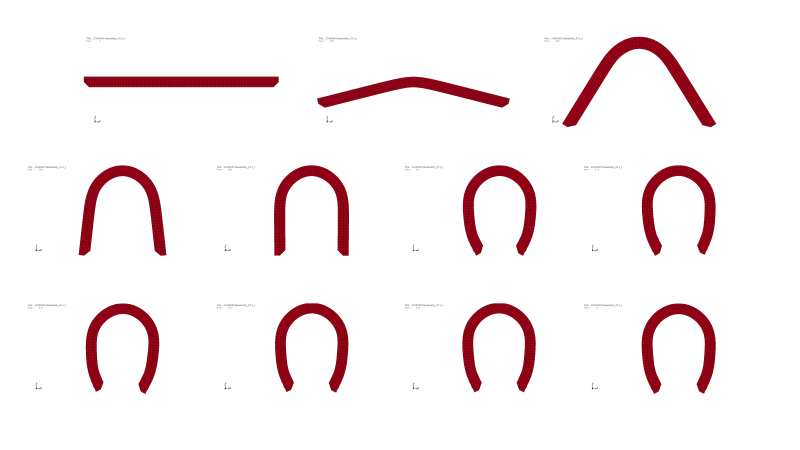
\includegraphics[width=0.95\textwidth]{src/ch4/shape_sequence_01.pdf}
\captionof{figure}{Secuencia de la geometría resultante}
\label{fig:shape_sequence_01}
\end{center}

\subsubsection{Esfuerzos}

\begin{center}
\includegraphics[width=0.75\textwidth]{src/ch4/von_mises_01.png}
\captionof{figure}{Distribución de esfuerzos de von Mises, final del primer paso}
\label{fig:von_mises_01}
\end{center}

\begin{center}
\includegraphics[width=0.75\textwidth]{src/ch4/von_mises_stress_01.pdf}
\captionof{figure}{Variación del esfuerzo máximo de von Mises}
\label{fig:von_mises_stress_01}
\end{center}

\begin{center}
\includegraphics[width=0.75\textwidth]{src/ch4/xyz_stress_01.pdf}
\captionof{figure}{Variación de los esfuerzos máximos en dirección X,Y,Z}
\label{fig:xyz_stress_01}
\end{center}



\subsubsection{Deformaciones}

\begin{center}
\includegraphics[width=0.75\textwidth]{src/ch4/efective_plastic_strain_01.png}
\captionof{figure}{Deformación plástica efectiva, final del primer paso}
\label{fig:efective_plastic_strain}
\end{center}

\begin{center}
\includegraphics[width=0.75\textwidth]{src/ch4/strain_x_01.png}
\captionof{figure}{Deformación en dirección X, final del primer paso}
\label{fig:efective_plastic_strain}
\end{center}

\begin{center}
\includegraphics[width=0.75\textwidth]{src/ch4/strain_y_01.png}
\captionof{figure}{Deformación en dirección Y, final del primer paso}
\label{fig:efective_plastic_strain}
\end{center}





\subsection{Análisis 3D}


\subsection{Estatus global}



\subsection{Esfuerzos}


\begin{center}
\includegraphics[width=0.75\textwidth]{src/ch4/von_mises_3D_01.png}
\captionof{figure}{Distribución del esfuerzo de von Mises}
\label{fig:von_mises_3D_01}
\end{center}

\begin{center}
\includegraphics[width=0.75\textwidth]{src/ch4/von_mises_3D_02.png}
\captionof{figure}{Distribución del esfuerzo de von Mises, segundo paso}
\label{fig:von_mises_3D_02}
\end{center}

\subsection{Deformaciones}

\begin{center}
\includegraphics[width=0.75\textwidth]{src/ch4/eqv_strain_01.png}
\captionof{figure}{Deformación plástica equivalente, primer paso}
\label{fig:eqv_strain_01}
\end{center}




\section{Del análisis experimemtal}


